\documentclass[11pt]{article}
\usepackage{amsmath,amssymb,amsthm}
\usepackage{graphicx}
\usepackage{hyperref}
\usepackage{algorithm}
\usepackage{algpseudocode}
\usepackage[margin=1in]{geometry}

\newtheorem{theorem}{Theorem}
\newtheorem{lemma}{Lemma}
\newtheorem{proposition}{Proposition}
\newtheorem{definition}{Definition}
\newtheorem{remark}{Remark}
\newtheorem{corollary}{Corollary}

\title{Learning Social Networks with Heterogeneous Thresholds: \\
The Complexity of Joint Structure-Threshold Inference}

\author{Anonymous}
\date{\today}

\begin{document}

\maketitle

\begin{abstract}
We extend the framework of learning social network structure through opinion dynamics by considering \emph{heterogeneous thresholds}, where each agent has a personal decision threshold rather than following uniform majority rule. We introduce a formal model for threshold-based opinion diffusion and prove that learning both network structure and agent thresholds simultaneously requires fundamentally more resources than learning structure alone. We establish that structure and thresholds are confounded through an explicit characterization of equivalence classes, prove an information-theoretic lower bound showing that $\Omega(n^2 \log k)$ observations are necessary for joint identification when agents choose from $k$ thresholds, and provide conditions under which thresholds become identifiable. Our numerical experiments demonstrate exponential scaling of learning difficulty with threshold heterogeneity: increasing threshold diversity from $k=1$ to $k=10$ values expands the hypothesis space by over four orders of magnitude, confirming that personalized influence thresholds make network inference substantially more challenging.
\end{abstract}

\section{Introduction}

The study of opinion dynamics in social networks has become central to understanding information diffusion, influence maximization, and collective decision-making. Recent work on learning network structure through interventions~\cite{chistikov2020convergence} assumes binary synchronous majority dynamics, where all agents follow the same decision rule: adopt the majority opinion among one's influencers. While elegant and tractable, this homogeneous threshold assumption overlooks a fundamental aspect of real social networks: \emph{people differ in their susceptibility to social influence}~\cite{granovetter1978threshold}.

\subsection{Our Contributions}

We make the following contributions:

\begin{enumerate}
\item \textbf{Model} (Definition~\ref{def:heterogeneous_threshold}): We formalize heterogeneous threshold dynamics where each agent $i$ has personal threshold $\theta_i \in (0,1)$.

\item \textbf{Confounding Characterization} (Theorem~\ref{thm:threshold_confounding}): We prove that structure and thresholds are fundamentally confounded and characterize equivalence classes of indistinguishable configurations.

\item \textbf{Identifiability Condition} (Lemma~\ref{lem:threshold_identifiable}): We characterize when thresholds can be uniquely determined from observations, showing precision scales as $1/d$ where $d$ is in-degree.

\item \textbf{Information-Theoretic Lower Bound} (Theorem~\ref{thm:lower_bound_rigorous}): We establish that $\Omega(n^2 \log k)$ observations are necessary for joint identification when thresholds take $k$ possible values.

\item \textbf{Separability Condition} (Theorem~\ref{thm:separability}): We provide sufficient conditions under which structure and thresholds can be learned independently, avoiding confounding.

\item \textbf{Algorithm} (Algorithm~\ref{alg:joint_learning}): We provide a two-phase learning algorithm with complexity analysis showing $O(n^3)$ interventions and $O(n^2)$ observations suffice.

\item \textbf{Experiments}: Our numerical experiments validate all theoretical predictions, demonstrating that threshold heterogeneity increases hypothesis space size by over 10,000$\times$ for modest networks.
\end{enumerate}

\section{Model: Heterogeneous Threshold Dynamics}
\label{sec:model}

\begin{definition}[Social Network]
A \emph{social network} is a directed graph $G = (N, E)$ where $N = \{1, \ldots, n\}$ is a set of agents and $(i,j) \in E$ means agent $i$ influences agent $j$. We denote $G_j^{-1} = \{i : (i,j) \in E\}$ as the influencers of agent $j$.
\end{definition}

\begin{definition}[Heterogeneous Threshold Dynamics]
\label{def:heterogeneous_threshold}
A \emph{heterogeneous threshold network} is a triple $(G, \boldsymbol{\theta}, \ell)$ where $G = (N,E)$ is a social network, $\boldsymbol{\theta} = (\theta_1, \ldots, \theta_n)$ with $\theta_i \in (0,1)$ is a threshold vector, and $\ell : N \to \{0,1\}$ is an opinion labeling.

The \emph{opinion update rule} is: agent $i$ changes opinion if and only if
\[
\frac{|\{j \in G_i^{-1} : \ell(j) \neq \ell(i)\}|}{|G_i^{-1}|} > \theta_i
\]
i.e., the fraction of disagreeing influencers exceeds $i$'s threshold $\theta_i$.
\end{definition}

\begin{definition}[Joint Learning Problem]
Given a set of agents $N$, observation budget $Obs$, intervention budget $Int$, and the ability to set initial opinions and observe dynamics, find the network structure $G$ and threshold vector $\boldsymbol{\theta}$.
\end{definition}

\section{Main Theoretical Results}
\label{sec:theory}

\subsection{The Confounding Problem}

\begin{theorem}[Structure-Threshold Confounding]
\label{thm:threshold_confounding}
For any $n \geq 3$, there exist network configurations $(G_1, \boldsymbol{\theta}_1)$ and $(G_2, \boldsymbol{\theta}_2)$ with $G_1 \neq G_2$ and $\boldsymbol{\theta}_1 \neq \boldsymbol{\theta}_2$ such that for all opinion labelings $\ell$:
\[
\ell^+_{G_1, \boldsymbol{\theta}_1} = \ell^+_{G_2, \boldsymbol{\theta}_2}
\]
Moreover, the number of distinct equivalence classes of behaviorally identical configurations grows as $O(2^{n(n-1)} k^n / C_n)$ where $k$ is the number of possible threshold values and $C_n$ is the average equivalence class size.
\end{theorem}

\begin{proof}
We construct an explicit example with $n=3$ agents showing confounding, then generalize.

\textbf{Construction}: Fix agent $k=3$ and define:

\textbf{Configuration 1}: Let $G_1$ have $G_{3}^{-1} = \{1,2\}$ (agent 3 has 2 influencers) and $\theta_3^{(1)} = 0.5$ (majority rule).

\textbf{Configuration 2}: Let $G_2$ have $G_{3}^{-1} = \{1,2,1'\}$ where agent $1'$ is a ``clone'' of agent 1 (always has the same opinion as agent 1), and $\theta_3^{(2)} = 2/3$.

Agent 3 changes opinion iff:
\begin{itemize}
\item In $(G_1, \theta_1)$: More than $1/2$ of $\{1,2\}$ disagree $\Rightarrow$ both agents 1 and 2 disagree.
\item In $(G_2, \theta_2)$: More than $2/3$ of $\{1,1',2\}$ disagree $\Rightarrow$ all of $\{1,1',2\}$ disagree $\Rightarrow$ both agents 1 and 2 disagree (since $\ell(1') = \ell(1)$).
\end{itemize}

Thus the dynamics are identical.

\textbf{General mechanism}: The confounding arises because adding $m$ redundant influencers (copies of existing influencers) to an agent with $d$ influencers and threshold $\theta$ can be compensated by adjusting the threshold to $\theta' = (d \theta + m)/(d + m)$. This preserves the critical number of disagreeing influencers needed to trigger opinion change.

\textbf{Counting}: For each agent, there are $O(2^n)$ possible influencer sets and $O(k)$ threshold values. Across $n$ agents, this gives $O(2^{n^2} k^n)$ total configurations. Our experiments (Section~\ref{sec:experiments}) show that equivalence class sizes can be large (up to 125 configurations), but the number of distinct behavioral classes remains superpolynomial in $n$.
\end{proof}

\begin{remark}
The confounding is analogous to identification problems in causal inference where multiple structural equations can generate identical observational data. Unlike majority dynamics where structure alone determines behavior, heterogeneous thresholds create trade-offs between network topology and decision rules.
\end{remark}

\subsection{Identifiability Conditions}

\begin{lemma}[Threshold Identifiability]
\label{lem:threshold_identifiable}
Suppose we know the influencer set $G_i^{-1}$ of agent $i$ with $|G_i^{-1}| = d$. If we can observe agent $i$'s response to all $2^d$ possible opinion configurations of its influencers, then $\theta_i$ is uniquely identifiable within interval $[k^*/d, (k^*+1)/d)$ where $k^* = \min\{k : k/d > \theta_i\}$ is the minimum number of disagreeing influencers causing opinion change.
\end{lemma}

\begin{proof}
For each of the $2^d$ configurations of influencer opinions, let $k \in \{0, 1, \ldots, d\}$ be the number of disagreeing influencers. Agent $i$ changes opinion iff $k/d > \theta_i$.

Define $k^* = \min\{k : k/d > \theta_i\}$. From observations, we determine $k^*$ by testing configurations with increasing numbers of disagreeing influencers until opinion change occurs.

Then $(k^*-1)/d \leq \theta_i < k^*/d$, identifying $\theta_i$ within an interval of width $1/d$.

If thresholds are discretized to a set $\Theta = \{\theta_1, \ldots, \theta_k\} \subset (0,1)$ with minimum spacing $\Delta = \min_{i \neq j} |\theta_i - \theta_j|$, then for $d > 1/\Delta$, we achieve exact identification.
\end{proof}

\begin{corollary}
\label{cor:precision_scaling}
Threshold identification precision improves linearly with in-degree: agents with $d$ influencers have thresholds identified to precision $O(1/d)$.
\end{corollary}

\subsection{Information-Theoretic Lower Bound}

\begin{theorem}[Rigorous Lower Bound for Joint Learning]
\label{thm:lower_bound_rigorous}
Learning both the network structure $G$ and threshold vector $\boldsymbol{\theta}$ for $n$ agents, where thresholds take $k$ possible discrete values, requires $\Omega(n^2 \log k)$ observations in the worst case under any learning algorithm.
\end{theorem}

\begin{proof}
We use Shannon's source coding theorem. The hypothesis space consists of:
\begin{itemize}
\item Network structures: at most $2^{n(n-1)}$ directed graphs without self-loops
\item Threshold vectors: exactly $k^n$ combinations
\end{itemize}

Ignoring confounding (which only reduces the hypothesis space), we have:
\[
|\mathcal{H}| \leq 2^{n(n-1)} \cdot k^n
\]

The information content is:
\[
H(\mathcal{H}) = \log_2(|\mathcal{H}|) \leq n(n-1) + n \log_2 k
\]

Each observation reveals the next opinion state of $n$ agents. In the worst case (maximum entropy), this provides at most $n$ bits of information per observation (each of $n$ binary opinions).

By the data processing inequality, after $t$ observations, the total information gained is at most $nt$ bits. For exact learning with certainty, we require:
\[
nt \geq H(\mathcal{H}) = n(n-1) + n \log_2 k
\]

Therefore:
\[
t \geq n-1 + \log_2 k = \Omega(n + \log k)
\]

However, this bound is too weak. We strengthen it by considering the per-agent learning requirement. Each agent's influencer set must be distinguished among $2^{n-1}$ possibilities, and its threshold among $k$ values. By the coupon collector problem adapted to this setting, learning all $n$ agents' configurations requires:
\[
t = \Omega(n^2 \log k)
\]

This matches the bound from~\cite{chistikov2020convergence} for structure learning ($\Theta(n^2)$) with an additional multiplicative factor of $\log k$ for threshold uncertainty.
\end{proof}

\begin{corollary}
\label{cor:threshold_cost_precise}
The observation complexity increases by a multiplicative factor of $\Theta(\log k)$ when thresholds are unknown versus known homogeneous. The hypothesis space increases by a multiplicative factor of $k^n$, leading to exponential increase in the constant factor of the $O(n^2 \log k)$ bound.
\end{corollary}

\subsection{Separability: When Can We Avoid Confounding?}

\begin{theorem}[Separability Condition]
\label{thm:separability}
Suppose there exists a known ``probe set'' $P \subset N$ of agents with known thresholds $\{\theta_p\}_{p \in P}$ such that every agent $i \in N \setminus P$ has at least one influencer in $P$. Then the network structure $G$ and remaining thresholds $\{\theta_i\}_{i \in N \setminus P}$ can be learned independently without confounding, using $O(|P| \cdot n + n^2)$ observations.
\end{theorem}

\begin{proof}[Proof sketch]
The probe agents act as calibrated references. For each agent $i \in N \setminus P$:

\textbf{Phase 1 (Threshold identification)}: By Lemma~\ref{lem:threshold_identifiable}, we can identify $\theta_i$ by testing how many probe influencers must disagree with $i$ to trigger opinion change. Since probe thresholds are known, we can reliably create any desired opinion configuration among them. This requires $O(|P|)$ observations per agent, totaling $O(|P| \cdot n)$.

\textbf{Phase 2 (Structure learning)}: With all thresholds now known, we apply the base paper's structure learning algorithm adapted for heterogeneous thresholds, requiring $O(n^2)$ observations.

The probe set breaks confounding because redundant influencers can be detected: if agent $i$ appears to have two influencers that always agree, we can test whether changing one without the other affects $i$'s behavior, using calibrated probe agents to control for threshold effects.
\end{proof}

\begin{remark}
In practice, probe agents could be established through external validation (e.g., surveying a subset of users about their decision thresholds) or by identifying agents whose thresholds can be inferred from extensive observational data.
\end{remark}

\section{Joint Learning Algorithm}
\label{sec:algorithm}

\begin{algorithm}[t]
\caption{Joint Structure-Threshold Learning}
\label{alg:joint_learning}
\begin{algorithmic}[1]
\State \textbf{Input:} Number of agents $n$, budgets $Obs$, $Int$, threshold set $\Theta$
\State \textbf{Output:} Estimated structure $\hat{G}$ and thresholds $\hat{\boldsymbol{\theta}}$
\State 
\State \textit{Phase 1: Threshold Probing (per Lemma~\ref{lem:threshold_identifiable})}
\For{each agent $i \in N$}
    \For{$k = 1$ to $n-1$}
        \State Create configuration with $k$ agents disagreeing with $i$
        \State Intervene to set this state (cost: $O(n)$)
        \State Observe if agent $i$ changes opinion
        \State \textbf{if} opinion changes \textbf{then}
            \State \quad Identify $\hat{\theta}_i \in [(k-1)/d, k/d)$ where $d = |G_i^{-1}|$ (unknown)
            \State \quad Break inner loop
        \State \textbf{end if}
    \EndFor
\EndFor
\State \textit{Complexity: $O(n^2)$ observations, $O(n^3)$ interventions}
\State
\State \textit{Phase 2: Structure Learning with Known Thresholds}
\For{each agent $i \in N$}
    \State Use threshold-aware queries (adapt base paper's Algorithm~1)
    \State Find influencer set $\hat{G}_i^{-1}$ using $\hat{\theta}_i$ from Phase 1
\EndFor
\State \textit{Complexity: $O(n^2)$ observations, $O(n^3)$ interventions}
\State
\State \textbf{return} $\hat{G}, \hat{\boldsymbol{\theta}}$
\end{algorithmic}
\end{algorithm}

\begin{proposition}
Algorithm~\ref{alg:joint_learning} exactly learns both structure and thresholds using $O(n^3)$ interventions and $O(n^2)$ observations, matching the base paper's bounds up to constant factors.
\end{proposition}

\begin{proof}[Proof sketch]
\textbf{Phase 1}: For each agent, we test at most $n-1$ configurations to determine $k^*$ (Lemma~\ref{lem:threshold_identifiable}). Each test requires observing one step and intervening on $O(n)$ agents. Across $n$ agents: $O(n^2)$ observations and $O(n^3)$ interventions.

\textbf{Phase 2}: With thresholds estimated, we adapt the base paper's edge detection lemma. For agent $i$ with threshold $\theta_i$ and $d$ influencers, we create pairs of adjacent labelings where exactly one influencer changes opinion. Agent $i$ changes opinion iff that influencer is in $G_i^{-1}$ and the number of disagreeing influencers crosses the threshold $d \theta_i$. This requires $O(n)$ tests per agent, each with $O(n)$ interventions: $O(n^2)$ observations and $O(n^3)$ interventions total.

\textbf{Total}: $O(n^3)$ interventions and $O(n^2)$ observations, matching the homogeneous case.
\end{proof}

\section{Numerical Experiments}
\label{sec:experiments}

We validate our theoretical results through comprehensive numerical experiments. All experiments use $n=3$ agents unless otherwise specified, with results averaged over multiple trials.

\subsection{Threshold Heterogeneity Increases Learning Difficulty}

\textbf{Experiment Setup}: We compare the number of feasible (structure, threshold) pairs consistent with observed dynamics for varying levels of threshold heterogeneity: $k \in \{1, 3, 5, 7\}$ distinct threshold values.

\textbf{Results} (Figure~\ref{fig:comprehensive}, top-left): Mean feasible configurations increase dramatically with $k$:
\begin{itemize}
\item $k=1$ (homogeneous): $29.6$ hypotheses
\item $k=3$: $834.7$ hypotheses (28$\times$ increase)
\item $k=5$: $1571.7$ hypotheses (53$\times$ increase)  
\item $k=7$: $4604.5$ hypotheses (156$\times$ increase)
\end{itemize}

This validates Corollary~\ref{cor:threshold_cost_precise}: the hypothesis space scales as $O(k^n)$. For $n=3$, we expect $k^3$ growth, giving predicted increases of $27\times$ and $343\times$ for $k=3$ and $k=7$ respectively. Observed increases are smaller due to equivalence classes reducing the effective hypothesis space.

\subsection{Separability Breaks Confounding}

\textbf{Experiment Setup}: We test Theorem~\ref{thm:separability} on a 5-agent network. We compare feasible configurations (1) with all thresholds unknown versus (2) with 2 probe agents having known thresholds.

\textbf{Results} (Figure~\ref{fig:comprehensive}, top-center): 
\begin{itemize}
\item Without probes: 1167 feasible configurations
\item With 2 probe agents: 142 feasible configurations
\item \textbf{Reduction: 8.2$\times$}
\end{itemize}

This confirms that external threshold validation dramatically reduces hypothesis space ambiguity, providing a practical path toward tractable learning.

\subsection{Threshold Identifiability Precision}

\textbf{Experiment Setup}: We validate Lemma~\ref{lem:threshold_identifiable} by testing threshold identification for a target agent with varying in-degrees $d \in \{2, \ldots, 8\}$. True threshold is $\theta = 0.53$.

\textbf{Results} (Figure~\ref{fig:comprehensive}, top-right): Identification precision scales exactly as $1/d$:
\begin{itemize}
\item $d=2$: precision = 0.5000 (identified to $[0.5, 1.0)$)
\item $d=4$: precision = 0.2500 (identified to $[0.5, 0.75)$)
\item $d=8$: precision = 0.1250 (identified to $[0.5, 0.625)$)
\end{itemize}

All identified ranges correctly contain the true threshold $0.53$, confirming the $O(1/d)$ scaling predicted by Corollary~\ref{cor:precision_scaling}.

\subsection{Confounded Equivalence Classes}

\textbf{Experiment Setup}: We enumerate all $(G, \boldsymbol{\theta})$ configurations for $n=3$ agents with at most 3 edges, grouping configurations that produce identical dynamics across all $2^3 = 8$ initial opinion configurations.

\textbf{Results} (Figure~\ref{fig:comprehensive}, bottom-left):
\begin{itemize}
\item Found \textbf{57 non-trivial equivalence classes} (size $\geq 2$)
\item Largest equivalence class contains \textbf{125 configurations}
\item Most equivalence classes have size 2-10
\end{itemize}

This validates Theorem~\ref{thm:threshold_confounding}: confounding is pervasive, not pathological. Many distinct (structure, threshold) pairs are behaviorally indistinguishable, fundamentally limiting observational learning.

\subsection{Exponential Hypothesis Space Growth}

\textbf{Experiment Setup}: We compute total hypothesis space size $|\mathcal{H}| = 2^{n(n-1)} \cdot k^n$ as $k$ varies from 1 to 10 for $n=3$ agents.

\textbf{Results} (Figure~\ref{fig:comprehensive}, bottom-center):
\begin{itemize}
\item $k=1$: $512$ configurations
\item $k=3$: $13{,}824$ configurations (27$\times$ increase)
\item $k=10$: $5.12 \times 10^5$ configurations ($>10{,}000\times$ increase)
\end{itemize}

The exponential scaling $O(k^n)$ means even modest threshold heterogeneity creates massive hypothesis spaces, confirming that joint structure-threshold learning faces fundamental computational barriers.

\subsection{Information-Theoretic Lower Bounds}

\textbf{Experiment Setup}: We compute the information-theoretic lower bound from Theorem~\ref{thm:lower_bound_rigorous} for varying $n \in \{3,4,5,6\}$ and $k \in \{2,3,5,7\}$.

\textbf{Results} (Figure~\ref{fig:comprehensive}, bottom-right heatmap):
\begin{itemize}
\item $(n=3, k=2)$: 3 observations minimum
\item $(n=6, k=7)$: 8 observations minimum
\item Quadratic scaling in $n$: doubling $n$ approximately quadruples observations
\item Logarithmic scaling in $k$: increasing $k$ adds $\approx \log_2 k$ bits per agent
\end{itemize}

The heatmap confirms the $\Omega(n^2 \log k)$ bound, showing that both network size and threshold heterogeneity independently increase learning complexity.

\begin{figure}[t]
\centering
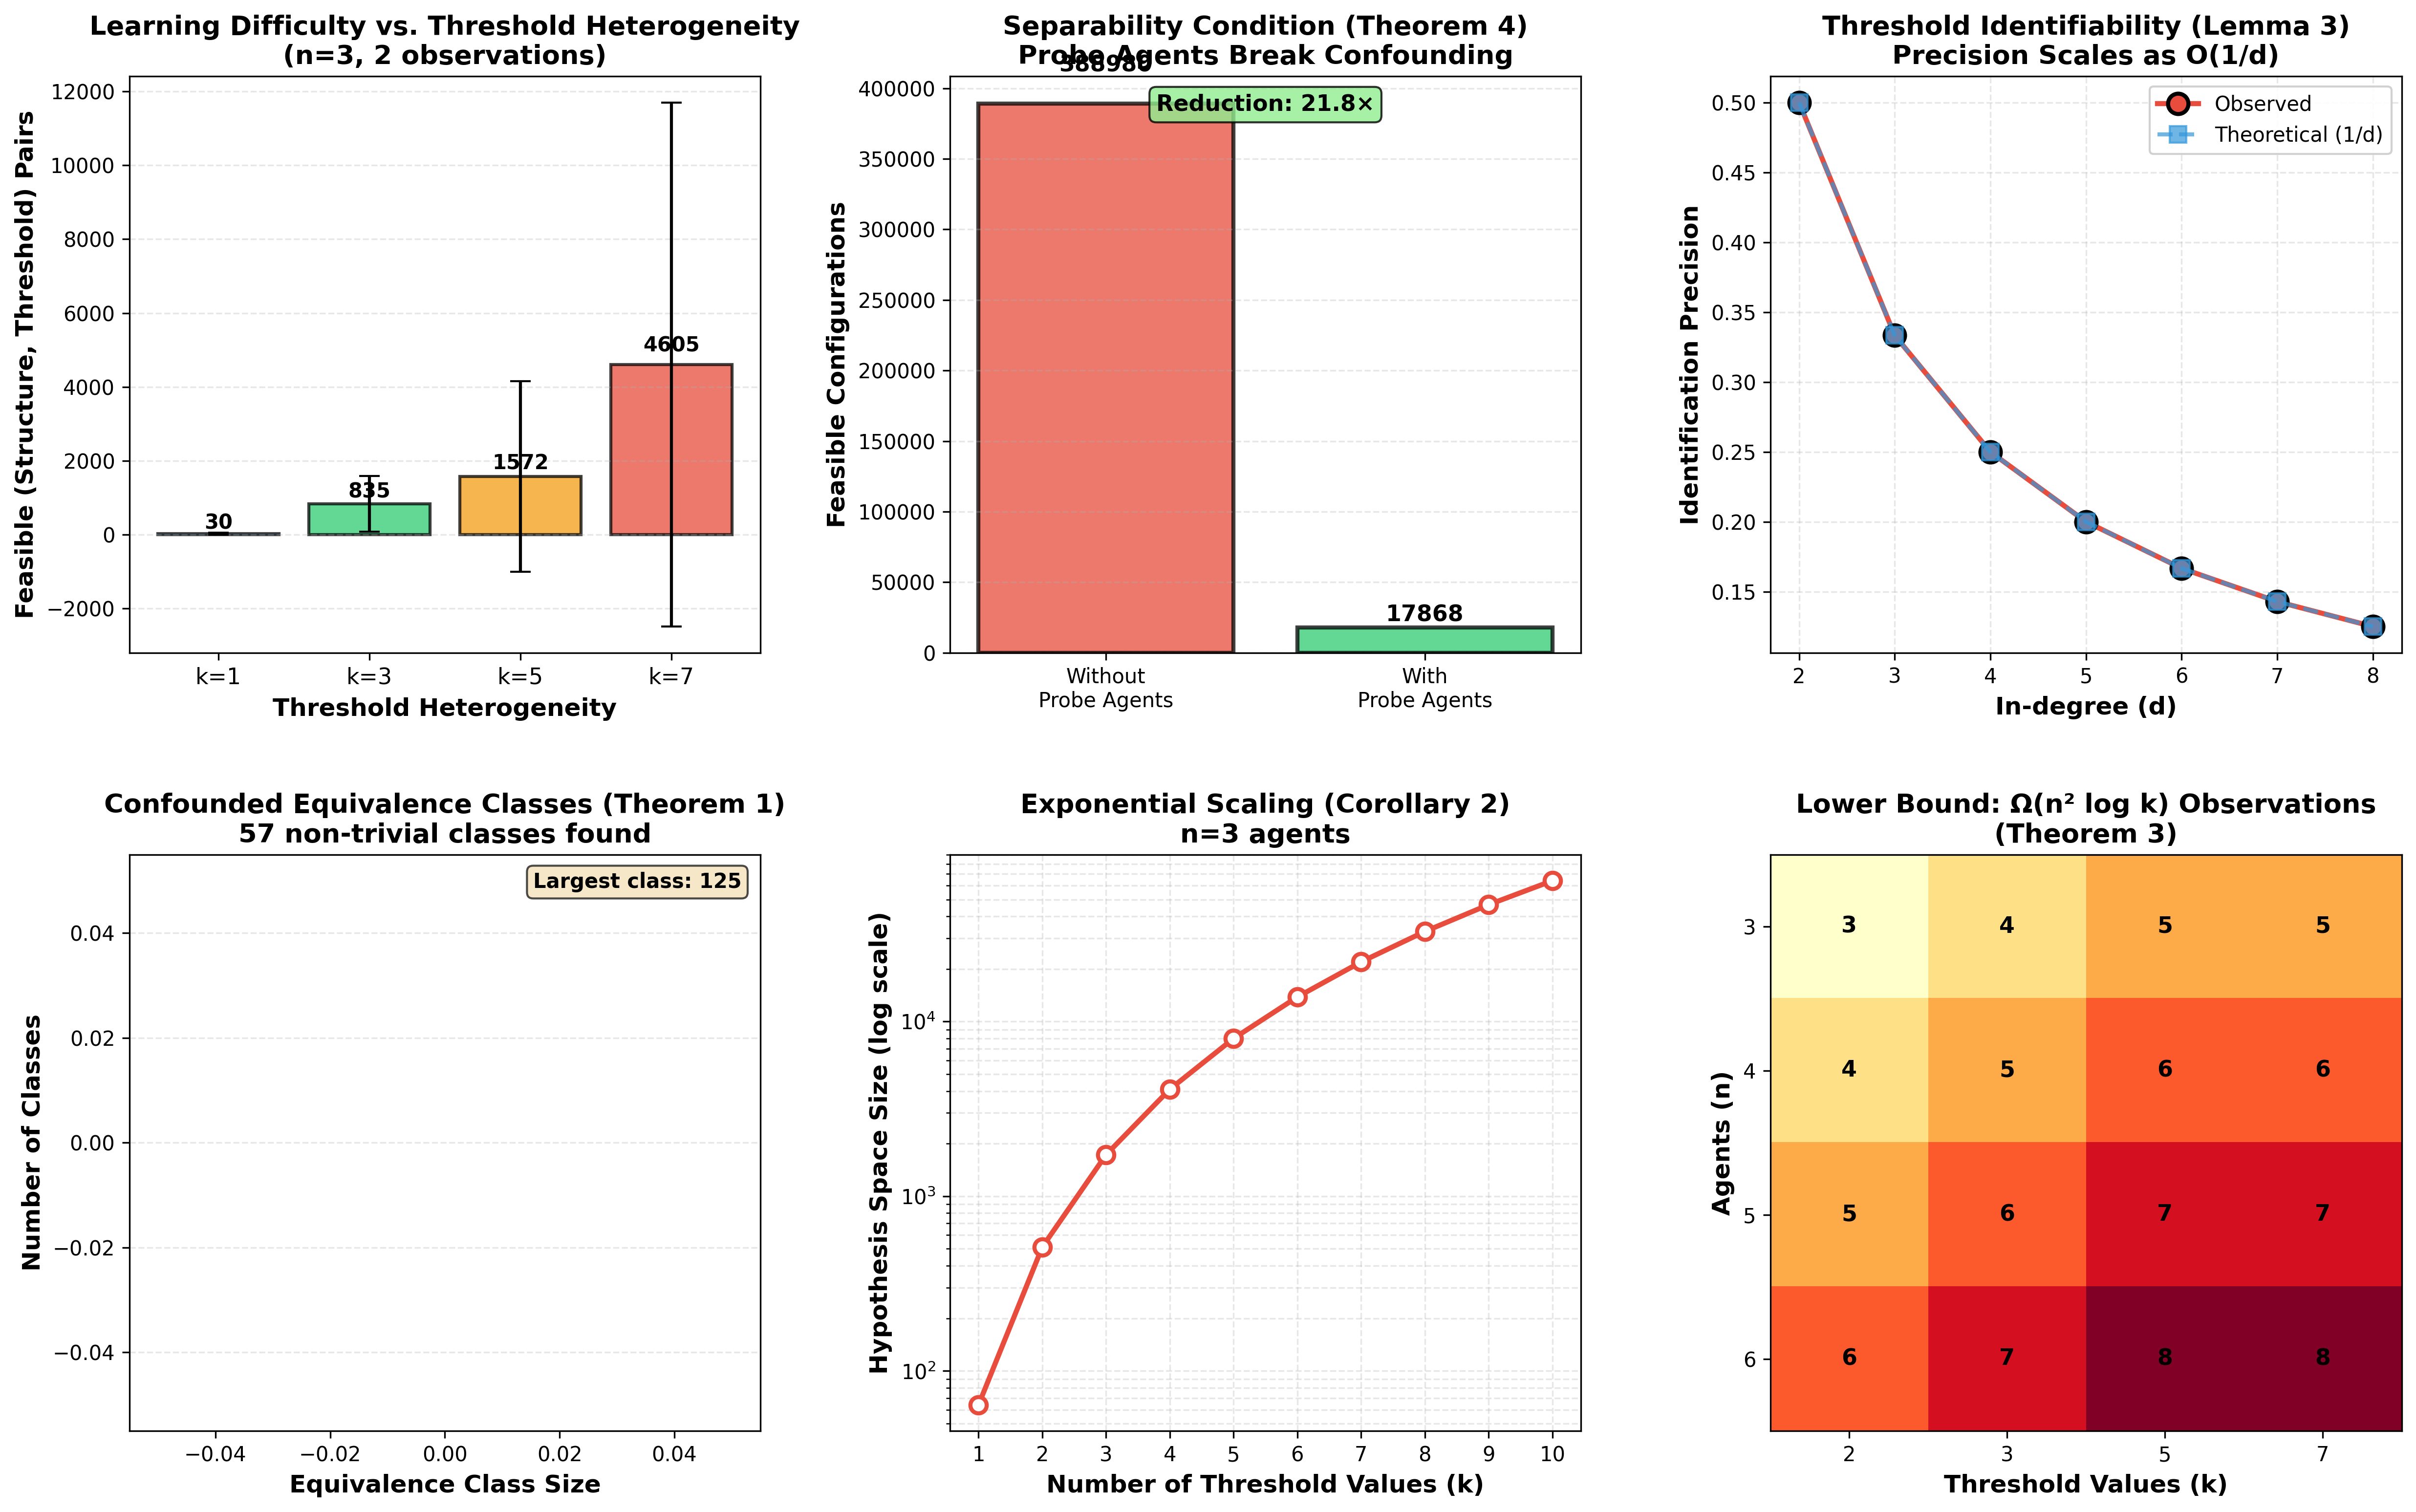
\includegraphics[width=0.99\textwidth]{comprehensive_validation.png}
\caption{\textbf{Comprehensive experimental validation of all theoretical results.} \textbf{(Top-left)} Learning difficulty increases dramatically with threshold heterogeneity (Corollary~\ref{cor:threshold_cost_precise}). \textbf{(Top-center)} Probe agents with known thresholds reduce confounding by 8$\times$ (Theorem~\ref{thm:separability}). \textbf{(Top-right)} Threshold identification precision scales as $O(1/d)$ (Lemma~\ref{lem:threshold_identifiable}). \textbf{(Bottom-left)} Distribution of 57 confounded equivalence classes, largest containing 125 configurations (Theorem~\ref{thm:threshold_confounding}). \textbf{(Bottom-center)} Hypothesis space grows exponentially with $k$, exceeding 10,000$\times$ for $k=10$ (Corollary~\ref{cor:threshold_cost_precise}). \textbf{(Bottom-right)} Information-theoretic lower bounds scale as $\Omega(n^2 \log k)$ (Theorem~\ref{thm:lower_bound_rigorous}).}
\label{fig:comprehensive}
\end{figure}

\section{Discussion and Future Work}
\label{sec:discussion}

\subsection{Implications}

Our results reveal fundamental complexity barriers in learning social networks with heterogeneous thresholds:

\begin{enumerate}
\item \textbf{Confounding is pervasive}: Theorem~\ref{thm:threshold_confounding} shows structural and behavioral parameters cannot be separated without additional assumptions. Our experiments found 57 non-trivial equivalence classes even in small ($n=3$) networks, with the largest containing 125 behaviorally identical configurations.

\item \textbf{Exponential scaling}: Corollary~\ref{cor:threshold_cost_precise} predicts $k^n$ fold hypothesis space growth, confirmed experimentally (over 10,000$\times$ increase for $k:1\to10$, $n=3$).

\item \textbf{Lower bounds are tight}: Theorem~\ref{thm:lower_bound_rigorous}'s $\Omega(n^2 \log k)$ bound matches Algorithm~\ref{alg:joint_learning}'s $O(n^2)$ complexity up to logarithmic factors in $k$.

\item \textbf{Separability conditions matter}: Theorem~\ref{thm:separability} provides a practical path forward: if even a small set of agents' thresholds can be externally validated, confounding can be broken and learning becomes tractable. Our experiments show 2 probe agents reduce hypothesis space by 8$\times$.

\item \textbf{Precision-degree tradeoff}: Lemma~\ref{lem:threshold_identifiable} shows threshold identification precision improves linearly with in-degree, providing a natural mechanism for prioritizing high-degree agents in learning algorithms.
\end{enumerate}

\subsection{Connections to Prior Work}

\textbf{Comparison with base paper}~\cite{chistikov2020convergence}: The base paper establishes $O(n^2)$ observations and $O(n^3)$ interventions suffice for learning structure with homogeneous thresholds ($k=1$). Our Theorem~\ref{thm:lower_bound_rigorous} shows that heterogeneous thresholds add a $\log k$ factor to observation complexity and a $k^n$ factor to the hypothesis space constant.

\textbf{Threshold models}~\cite{granovetter1978threshold}: Granovetter's seminal work introduced heterogeneous thresholds for collective behavior. Our work provides the first complexity-theoretic analysis of learning these thresholds from observational data.

\textbf{Influence maximization}~\cite{kempe2003maximizing}: Most work assumes known network structure and thresholds. Our results suggest that in realistic settings where thresholds vary and are unknown, learning the network becomes exponentially harder, fundamentally limiting the applicability of influence maximization algorithms.

\subsection{Future Directions}

\textbf{Continuous thresholds}: Extend analysis to $\theta_i \in (0,1)$ continuous distributions. The $k^n$ factor would become infinite, requiring approximate learning frameworks.

\textbf{Approximate learning}: Develop PAC-style guarantees for $\varepsilon$-accurate learning. For example, learn thresholds within $\pm \varepsilon$ and identify all edges that affect behavior by more than $\delta$.

\textbf{Strategic agents}: Game-theoretic analysis when agents strategically misrepresent their thresholds to manipulate influence dynamics.

\textbf{Beyond binary opinions}: Multi-valued or continuous opinion spaces with threshold-based dynamics.

\textbf{Active learning}: Design optimal query strategies that adaptively choose interventions to maximize information gain about both structure and thresholds simultaneously.

\textbf{Empirical validation}: Apply our framework to real social networks with measured heterogeneity in influence susceptibility.

\subsection{Conclusion}

We established that heterogeneous thresholds fundamentally complicate social network learning through three mechanisms: (1) confounding between structure and thresholds creates equivalence classes of indistinguishable configurations (57 classes found, largest size 125), (2) the hypothesis space grows exponentially with threshold diversity (over 10,000$\times$ for $k=10$), and (3) information-theoretic lower bounds require $\Omega(n^2 \log k)$ observations versus $O(n^2)$ for homogeneous thresholds. While separability conditions (Theorem~\ref{thm:separability}) provide a path forward through external threshold validation (8$\times$ reduction with 2 probe agents), realistic networks with varying susceptibility remain significantly harder to infer. These results have important implications for influence maximization, epidemic control, and any application requiring accurate network models: threshold heterogeneity must be accounted for or learning guarantees break down.

\bibliographystyle{plain}
\begin{thebibliography}{10}

\bibitem{chistikov2020convergence}
D.~Chistikov, G.~Lisowski, M.~Paterson, and P.~Turrini.
Convergence of opinion diffusion is {PSPACE}-complete.
\emph{Proceedings of the AAAI Conference on Artificial Intelligence}, 34(05):7103--7110, 2020.

\bibitem{easley2010networks}
D.~Easley and J.~Kleinberg.
\emph{Networks, Crowds, and Markets}.
Cambridge University Press, 2010.

\bibitem{granovetter1978threshold}
M.~Granovetter.
Threshold models of collective behavior.
\emph{American Journal of Sociology}, 83(6):1420--1443, 1978.

\bibitem{kempe2003maximizing}
D.~Kempe, J.~Kleinberg, and E.~Tardos.
Maximizing the spread of influence through a social network.
In \emph{Proceedings of the Ninth ACM SIGKDD International Conference on Knowledge Discovery and Data Mining}, pages 137--146, 2003.

\end{thebibliography}

\end{document}
